\subsection{Angular distribution and observables}
\label{sec:kpimm:angular-distribution}

\begin{figure}
\centering
\begin{subfigure}{0.49\textwidth}
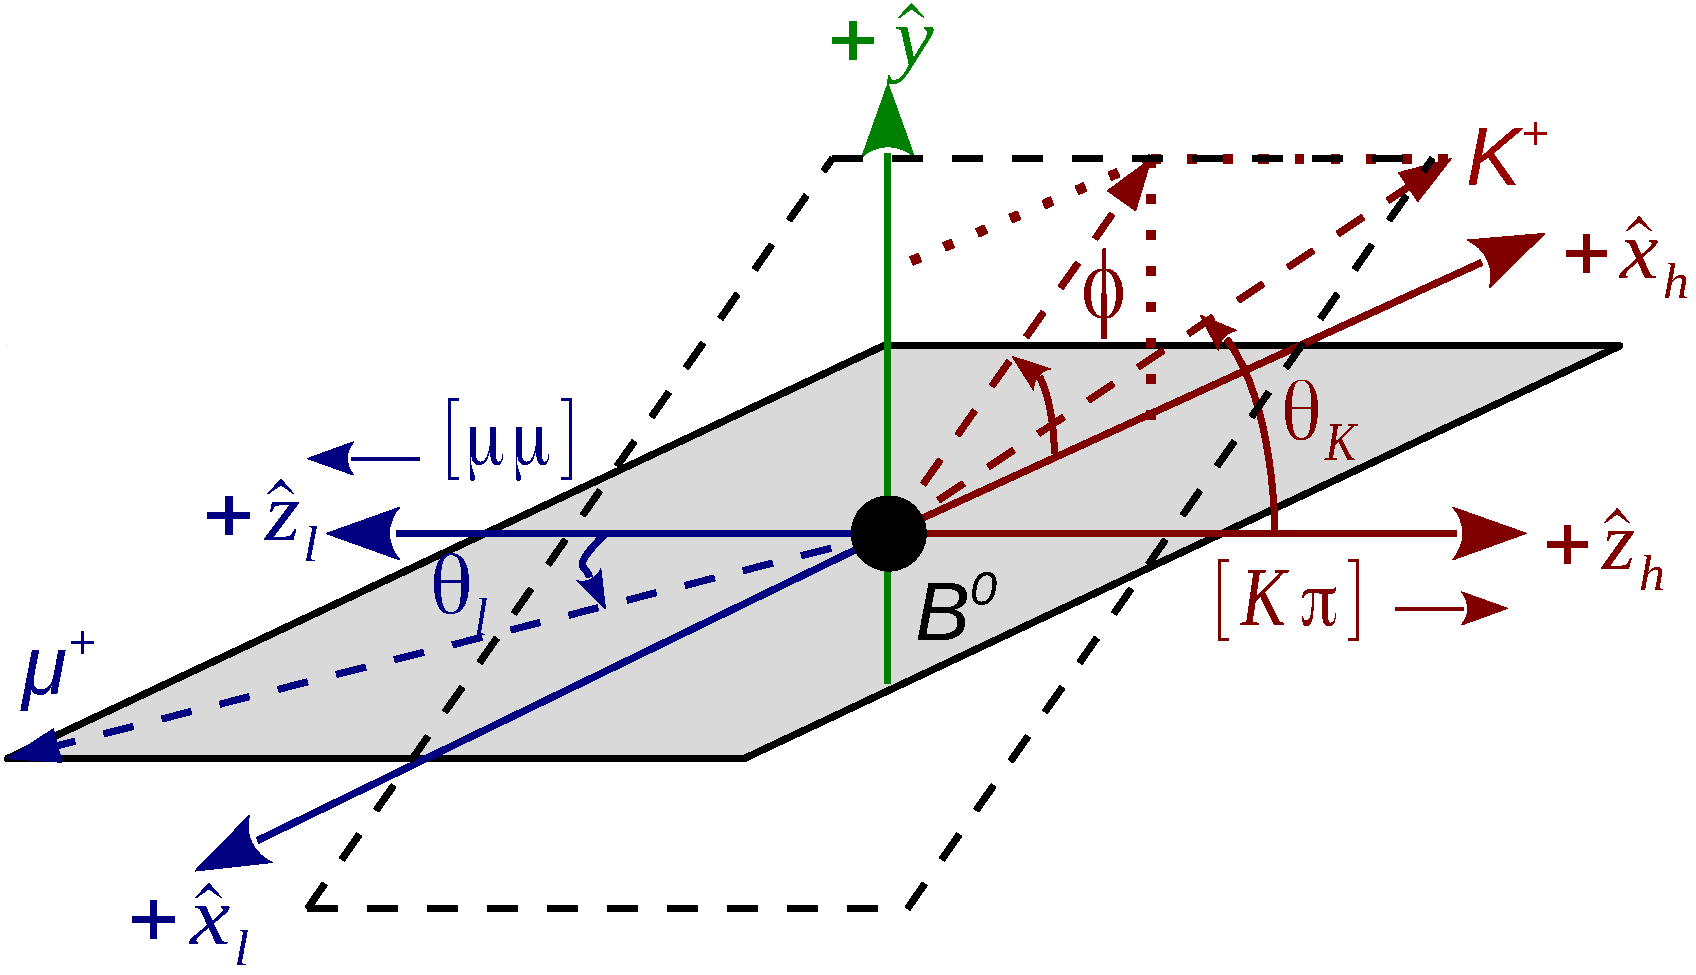
\includegraphics[width=\textwidth]{figs/kpimm/angular-distribution/angles_bz.pdf}
\caption{}
\label{fig:angle_conventions:bzb}
\end{subfigure}
\begin{subfigure}{0.49\textwidth}
\centering
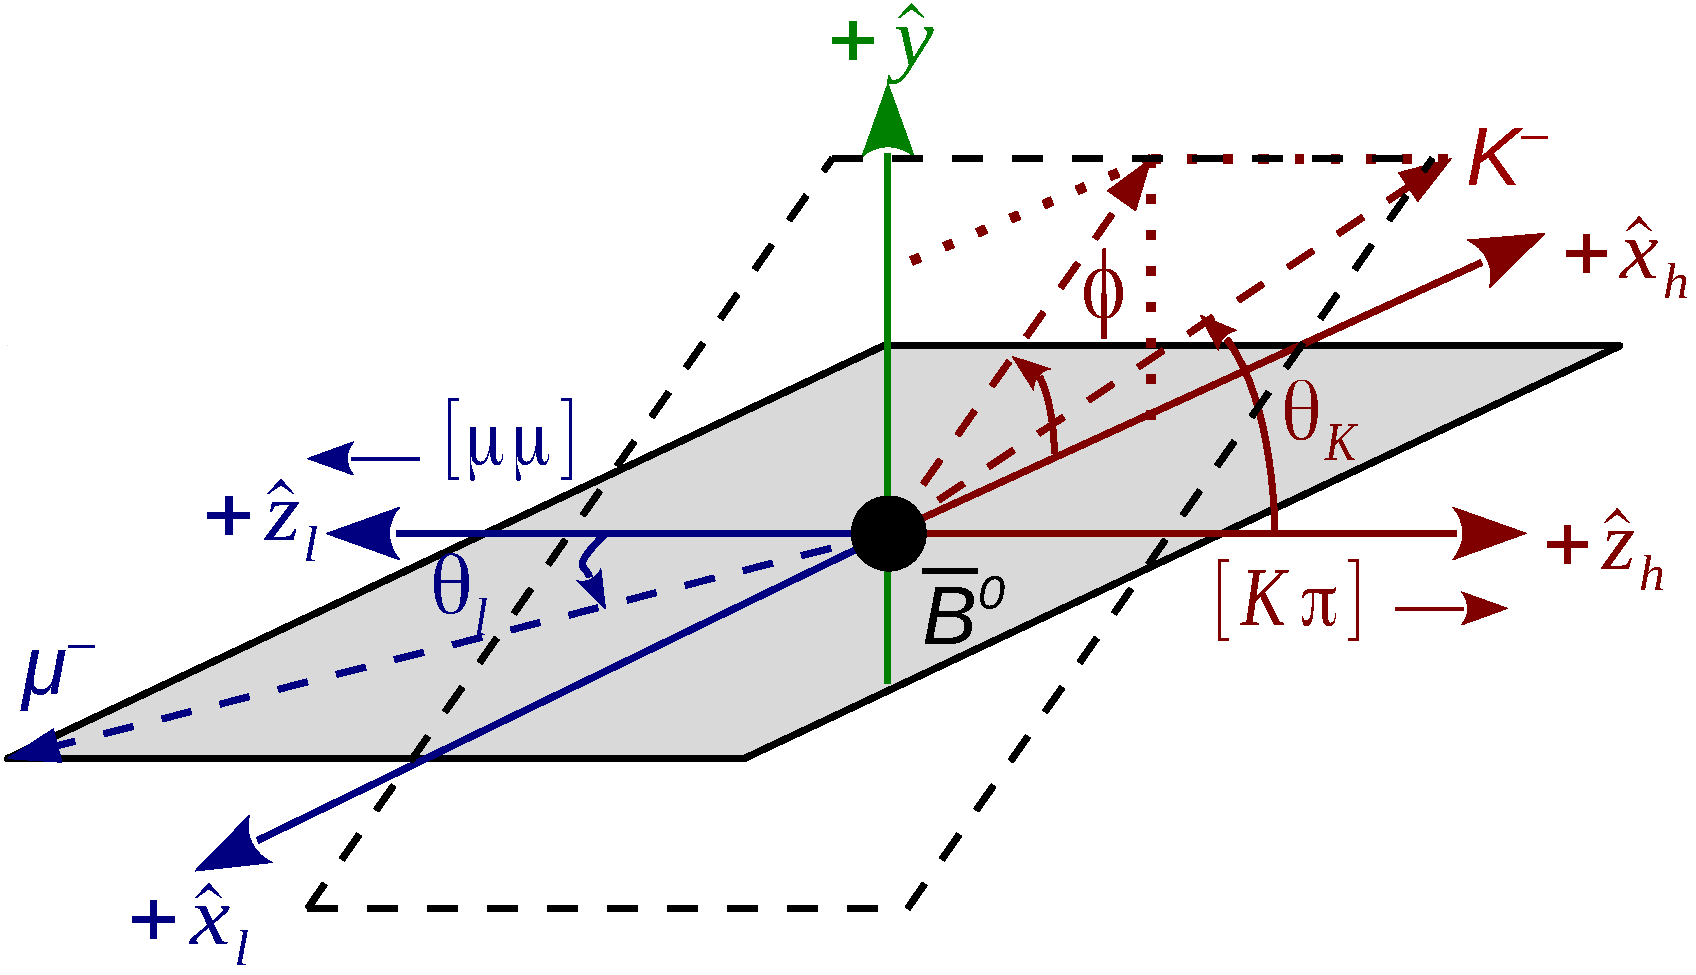
\includegraphics[width=\textwidth]{figs/kpimm/angular-distribution/angles_bzb.pdf}
\caption{}
\label{fig:angle_conventions:bz}
\end{subfigure}
\caption{Angle conventions for the (a) $\Bzb \to \Km \pip \mun \mup$ (b)  $\Bz \to \Kp \pim \mup \mun$ as described in Ref.~\cite{biplab}. The leptonic and hadronic frames are back-to-back with a common $\hat{y}$ axis. For the dihedral angle $\phi$ between the leptonic and hadronic decay planes, there is an additional sign flip $\phi\to -\phi$ compared to previous \lhcb analyses~\cite{LHCB-PAPER-2011-020,LHCB-PAPER-2013-019,LHCB-PAPER-2013-037,LHCB-PAPER-2015-051}.
}
\label{fig:angle_conventions}
\end{figure}

The final state of the decay \BdToKpimm is fully described by five kinematic variables: three decay angles (\thetal, \thetak, $\phi$); \mkpi, the invariant mass of the \Kp\pim system; and \qsq, the invariant mass squared of the dimuon system. 
Figure~\ref{fig:angle_conventions:bzb} shows the angle conventions for the $\Bzb$ decay (containing a \bquark quark): the back-to-back leptonic and hadronic systems share a common $\hat{y}$ axis and have opposite $\hat{x}$ and $\hat{z}$ axes. 
The negatively charged lepton is used to define the leptonic helicity angle $\thetal$ for the $\Bzb$.
The quadrant of the dihedral angle $\phi$ between the dimuon and the $\Kstarz \to K\pi$ decay planes is set by requiring the azimuthal angle of the $\mun$ to be zero in the leptonic helicity frame. The azimuthal angle of the $\Km$ in the hadronic helicity frame is then equal to $\phi$. Compared to the dihedral angle used in the previous \lhcb analyses~\cite{LHCB-PAPER-2011-020,LHCB-PAPER-2013-019,LHCB-PAPER-2013-037,LHCB-PAPER-2015-051}, there is an additional sign flip $\phi \to -\phi$ in the convention used in this analysis. For the $\Bz$ decay (containing a \bquarkbar-quark), the charge conjugation is performed explicitly, and the angles are shown in Fig.~\ref{fig:angle_conventions:bz}. That is, for the $\Bz$, the $\mup$ and $\Kp$ directions are used to define the angles. In the absence of direct \CP violation, to keep the measured angular observables the same between the $\Bzb$ and $\Bz$, an additional minus sign is added to the dihedral angle when performing the \CP conjugation.

In the limit where the muon mass squared is small compared to $\qsq$, the \CP averaged differential decay rate of \BdToKpimm decays with the \Kp\pim system in a S-, P-, or D-wave configuration, outlined in Ref.~\cite{biplab}, can be expanded in an orthonormal basis of angular functions $f_i(\Omega)$ as

\begin{equation}
\label{eqn:vector_moments}
\frac{\deriv\Gamma }{\deriv\qsq \deriv\Omega} = \mathcal{C} \times \left\{ \displaystyle \sum^{41}_{i=1} f_i (\Omega) \Gamma_i(\qsq) \right\} 
 \quad\mbox{with}\quad
\Gamma_i(\qsq) = \Gamma^L_i(\qsq) + \eta^{L\to R}_i\; \Gamma^R_i(\qsq),
\end{equation}

\noindent where $\mathcal{C}$ is a pre-factor, $\deriv\Omega = \deriv\ctl \deriv\ctk \deriv\phi$, and $L$ and $R$ denote the (left- and right-handed) chirality of the lepton system. The sign $\eta^{L\to R}_i=\pm 1$ depends on the signature of $f_i$ under $\thetal \to \pi + \thetal$. 
\noindent The orthonormal angular basis is constructed out of the spherical harmonics, \mbox{$Y^m_l \equiv Y^m_l (\thetal,\phi)$}, and the reduced spherical harmonics, \mbox{${P^m_l \equiv \sqrt{2 \pi}Y^m_l(\thetak,0)}$}.
 
The transversity-basis moments of the 41 orthonormal angular functions are given in Appendix~\ref{sec:appendix:angular-distribution}. The convention is that the amplitudes correspond to the $\Bzb$ decay. The S-, P- and D-wave transversity amplitudes are denoted as $S^{\{L,R\}}$, $H^{\{L,R\}}_{\{0,\parallel,\perp\}}$ and $D^{\{L,R\}}_{\{0,\parallel,\perp\}}$, respectively. 

The measured angular observables are averaged over the range $1330<\mkpi<1530~\mevcc$ and $1.1<\qsq<6.0\gevgevcccc$. The choice of $\qsq$ region pertains to the so-called large-recoil regime where the recoiling daughter meson has a relatively large energy, $E_{K^\ast}$, in the rest-frame of the parent $B$ meson. In the limit $\Lambda_{\rm QCD}/E_{K^\ast} \to 0$, the uncertainties arising from hadronic effects in the relevant form-factors are reduced at leading order, leading to more reliable theory predictions~\cite{DescotesGenon:2013wba}. The high-$\qsq$ region above the $\psi(2S)$ resonance is polluted by broad charmonium resonances and is also phase-space suppressed for higher \mkpi masses. Therefore, this region is not considered in this study.

In the present analysis, the first moment, $\Gamma_{1}(\qsq)$, corresponds to the total rate. From the total rate, 40 normalised moments with $i \in \{2,...,41\}$ are defined as
\begin{equation}
\label{eqn:norm_mom_def}
\overline{\Gamma}_i(\qsq) = \frac{\Gamma_{i}(\qsq)}{\Gamma_{1}(\qsq)}.
\end{equation}
\noindent These form the set of observables that are measured in the angular moments analysis described in Sec.~\ref{sec:kpimm:angular-analysis}.